% 1- Explicar detenidamente la principal motivacion del articulo. Dejar claro cual es el posible problema
% 2- Presentar las preguntas de investigacion pertinentes
% 3- Presentar algunos resultados preliminares
% 4- Presentar el trabajo llevado hasta ahora de investigacion y desarrollo
% 5- Dejar algunas preguntas abiertas y problemas encontrados hasta ahora
%
% $Id: slides.tex 4228 2006-06-21 21:55:12Z jjamor $
%
%
% Compilar a .pdf con LaTeX (pdflatex)
% Es necesario instalar Beamer (paquete latex-beamer en Debian)
%

%
% Grficos:
% Los grficos pueden suministrarse en PNG, JPG, TIF, PDF, MPS
% Los EPS deben convertirse a PDF (usar epstopdf)
%


\documentclass{beamer}
\usetheme{Warsaw}
\usebackgroundtemplate{
\includegraphics[width=\paperwidth]{format/libresoft-bg.png}}
\usepackage[english]{babel}
\usepackage[utf8]{inputenc}
\usepackage{graphics}
\usepackage{amssymb} % Simbolos matematicos
\usepackage{url}

%\definecolor{libresoftgreen}{RGB}{162,190,43}
%\definecolor{libresoftblue}{RGB}{0,98,143}

%\setbeamercolor{titlelike}{bg=libresoftgreen}

%% Metadatos del PDF.
\hypersetup{
  pdftitle={Libresoft},
  pdfauthor={Daniel Izquierdo Cort\'azar},
  pdfcreator={GSyC/Libresoft},
  pdfproducer=PDFLaTeX,
  pdfsubject={Exercise: Ohloh community metrics},
}
%%



\AtBeginSection[]
{
  \begin{frame}<presentation>
    \frametitle{Index}
    \tableofcontents[current]
  \end{frame}
}




\begin{document}



\title{Ohloh community metrics
}
\subtitle{ Master on Free Software
}
\institute{jfelipe@libresoft.es\\
GSyC/Libresoft, Universidad Rey Juan Carlos}
\author{Felipe Ortega, Pedro Coca, Daniel Izquierdo Cort\'azar}
\date{Fuenlabrada, Madrid\\ 2nd, December 2010}

\frame{
\maketitle
\begin{center}

\includegraphics[width=4cm]{format/gsyc-urjc.pdf} 
\end{center}
}


% Si el titulo o el autor se quieren acortar para los pies de pgina
% se pueden redefinir aqu:
%\title{Titulo corto}
%\author{Autores abreviado}


%% LICENCIA DE REDISTRIBUCION DE LAS TRANSPAS
\frame{
~
\vspace{4cm}

\begin{flushright}
{\tiny
(cc) 2010 Felipe Ortega. \\
Some rights reserved. This document is distributed under the Creative \\
            Commons Attribution-ShareAlike 3.0 licence, available in \\
            http://creativecommons.org/licenses/by-sa/3.0/

%  Este documento (o uno muy similar) está disponible en \\
%  \url{http://gsyc.escet.urjc.es/~jjamor/}
}
\end{flushright}
}
%%

\frame{
\frametitle{Table of contents}
\tableofcontents
}


\section{Introduction}


\begin{frame}
\frametitle{Motivation}
\begin{center}
\begin{itemize}
\item Community driven metrics about projects.
\item Includes plain analysis and also assesment about project quality
\item Interesting mix:
\begin{itemize}
 \item Automated analyses (oh-count, oh-scm)
 \item Community feedback (who develops what, check analyses results).
\end{itemize}
\end{itemize}
\end{center}
\end{frame}

\section{Features}

\begin{frame}
\frametitle{List of high-level features}
\begin{center}
\begin{itemize}
 \item Project comparison
 \item Language comparison
 \item Repositories comparison
\end{itemize}

\end{center}
\end{frame}

\begin{frame}
\frametitle{Repositories comparison in Ohloh}
\begin{center}
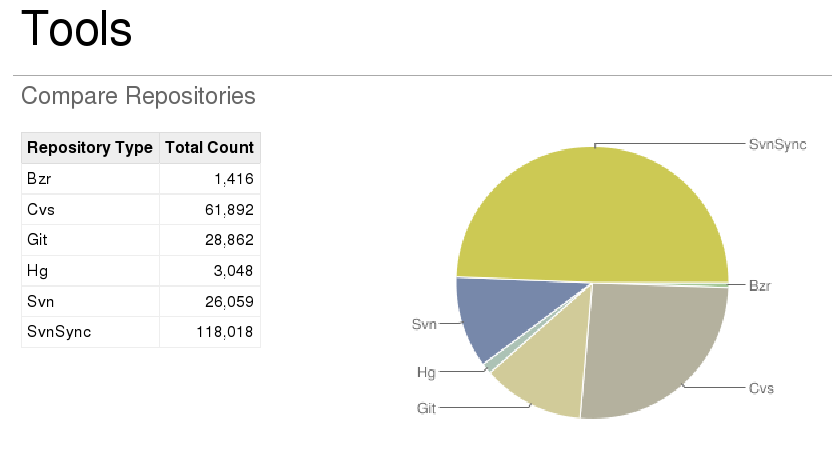
\includegraphics[width=0.9\textwidth]{figs/ohloh-repos-comparison.png}
\end{center}
\end{frame}

\begin{frame}
\frametitle{Projects' factsheet}
\begin{center}
\begin{itemize}
 \item Quantitative analysis.
 \item Quality assessment.
 \item Many other features... some difficult to find elsewhere.
 \item \scriptsize{\texttt{http://www.ohloh.net/announcements/source\_license\_detector\_released}}
\end{itemize}
\end{center}
\end{frame}

\section{Examples}

\begin{frame}
\frametitle{Firefox in Ohloh}
\begin{center}
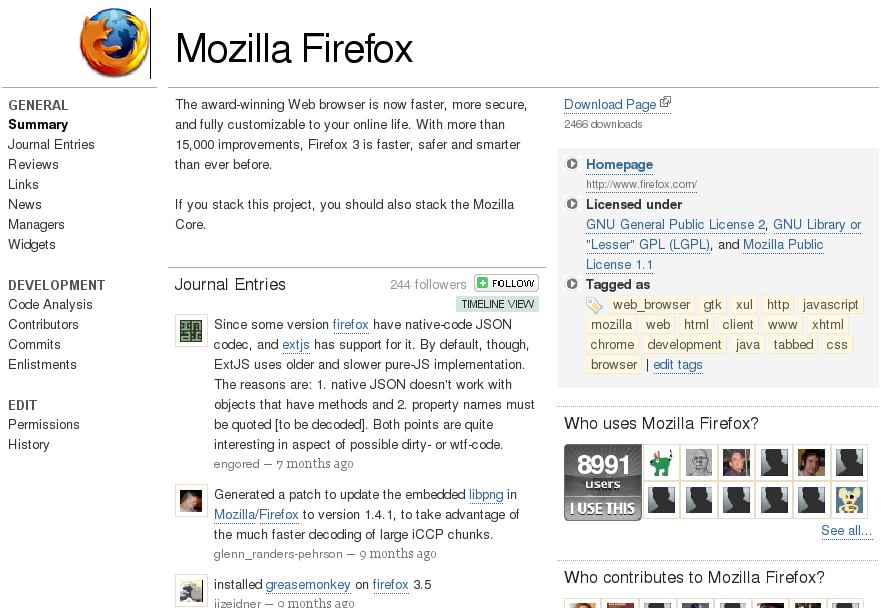
\includegraphics[width=0.8\textwidth]{figs/ohloh-firefox.png}
\end{center}
\end{frame}

\begin{frame}
\frametitle{Evince in Ohloh}
\begin{center}
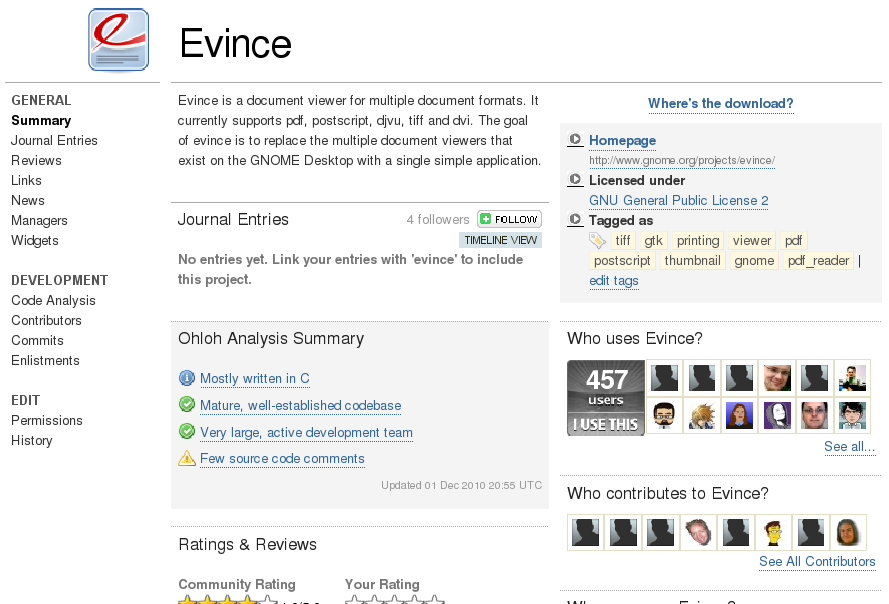
\includegraphics[width=0.9\textwidth]{figs/ohloh-evince.png}
\end{center}
\end{frame}

\begin{frame}
\frametitle{Kmail in Ohloh}
\begin{center}
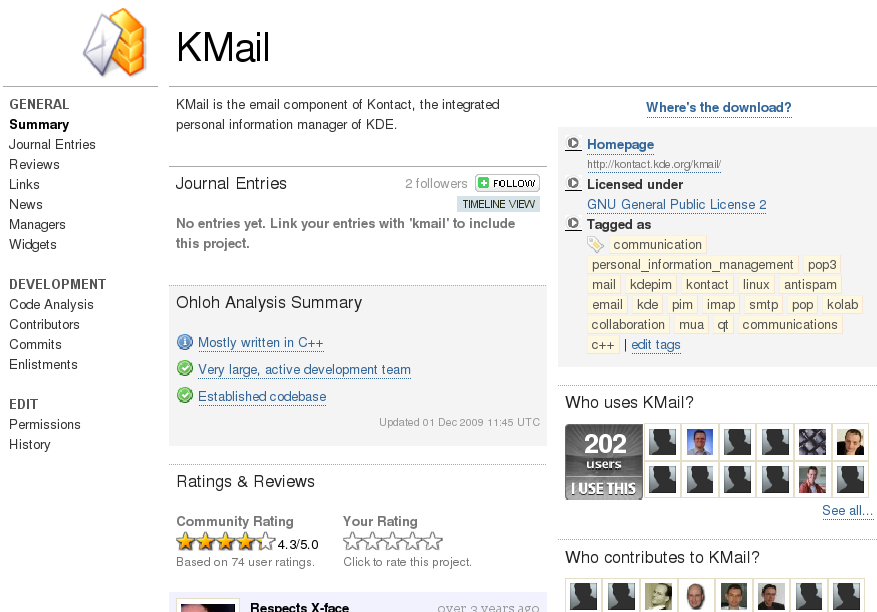
\includegraphics[width=0.9\textwidth]{figs/ohloh-kmail.png}
\end{center}
\end{frame}

\section{Activity}

\begin{frame}
\frametitle{Explore Ohloh's metrics and goals}
\begin{center}
\begin{itemize}
 \item Gather a complete list of project metrics
 \item How can users contribute back to the platform?
 \item How can they check analysis results?
 \item How can Ohloh offer quality assessments based on these results?
 \item Would you find this info useful to assess the quality of a FLOSS project?
 \item Would you rely on this info to select a FLOSS project to cover a specific need of your company?
\end{itemize}
\end{center}
\end{frame}

\end{document}
